

Although we advocate mass-mass plots as the primary 
presentation of  LHC results, it is nevertheless interesting and informative to compare  the LHC limits with the results from other DM searches. To avoid the difficulties associated with reinterpreting the results of non-collider experiments, we recommend translating the LHC results onto the plots of non-collider experiments, rather than the reverse procedure. When performing a translation to the non-collider planes, it is important to bear in mind the different underlying assumptions.  While the DD or ID bounds may be valid for multiple DM models, the LHC limits hold exclusively for the mediator under investigation and for the specific choices of the couplings used in the simplified model.

For a given mediator the translation procedure is well-defined. In this section, we explain all of the ingredients needed for a correct translation into the cross section-mass planes in which  DD and ID experiments present their results. As input, we use  LHC bounds in the mass-mass plane for fixed couplings~$\gSM$ and~$\gDM$ (see Section~\ref{sec:colliderresults}). To compare with  DD experiments, these limits are translated into the  planes of the DM mass $\mDM$ versus the spin-independent (SI) or spin-dependent (SD)  DM-nucleon cross section, $\sigma_{\rm SI}$ or~$\sigma_{\rm SD}$. For a comparison with ID experiments, the limits are instead converted into the plane defined by $\mDM$ and the DM annihilation cross section $\sigv$.

\subsection{ DD experiments}

DD experiments search for the recoil of a nucleus scattering off a DM particle traversing the detector. Since the DM particle is non-relativistic, the dominant interactions between DM and nuclei can be described by two effective parameters, namely the SI and SD DM-nucleon scattering cross sections. DD experiments present their limits as bounds on these  cross section as a function of $\mDM$, where common units for the  cross section are either $\text{cm}^2$ or~pb. The  bounds are presented at 90\%~CL, as opposed to the 95\%~CL limits that are the standard in the collider community. For the sake of comparison, we recommend to present the  LHC limits on the  $\mDM$--$\hspace{0.25mm} \sigma_{\rm{SI/SD}}$ planes at 90\%~CL.

In principle, it is necessary to distinguish between the DM-proton scattering cross sections  $\sigma^p_{\rm{SI}/\rm{SD}}$ and the DM-neutron scattering cross sections  $\sigma^n_{\rm{SI}/\rm{SD}}$. For  SI interactions, however,  DD bounds are always shown under the assumption that $\sigma^p_{\rm{SI}} = \sigma^n_{\rm{SI}}$, which also holds for the simplified models proposed here. For  SD interactions it is common to present separate bounds on $\sigma^p_{\rm{SD}}$ and $\sigma^n_{\rm{SD}}$ and it is possible to compare  LHC results with both.

There are currently a rather large number of  DD experiments that have different target nuclei and use different detection technologies. For  SI interactions, the most sensitive experiments for DM particles heavier than $\mathcal{O}(10 \, \mathrm{GeV})$ are two-phase xenon experiments. There are two large competing collaborations employing this technology, LUX~\cite{Akerib:2015rjg} and XENON1T~\cite{Aprile:2015uzo} (previously XENON100). LUX has published results from its first run and is currently collecting more data to improve its sensitivity. XENON1T will soon begin its first run and aims to have first results in late 2016. For DM particles lighter than $\mathcal{O}(10 \, \mathrm{GeV})$, solid state cryogenic detectors as used by the SuperCDMS~\cite{Agnese:2015nto} and CRESST-II~\cite{Angloher:2015ewa} collaborations are more constraining than xenon experiments as their energy threshold is lower.

As mentioned above, for  SD interactions, separate bounds are published on $\sigma^p_{\rm{SD}}$ and~$\sigma^n_{\rm{SD}}$. This is because DM scatters with the spin of the isotope which is approximately due to an unpaired neutron or unpaired proton. In practice this means that DD experiments have good sensitivity to $\sigma^p_{\rm{SD}}$ or $\sigma^n_{\rm{SD}}$ but not both. The strongest DD limits on~$\sigma^p_{\rm{SD}}$ are from the PICO collaboration~\cite{Amole:2016pye,Amole:2015pla}, while the strongest limits on $\sigma^n_{\rm{SD}}$ are from LUX~\cite{Akerib:2016lao}.\footnote{Note an open source data resource where many DD experiments have uploaded limits is {\tt DMTools}~\cite{DMTools}. These data, however, are not always officially blessed or scrutinised by the experiments and thus should be used with care.}


The simplified models with a vector and scalar mediator lead to a SI interaction, while the axial-vector and  pseudo-scalar mediator induce SD interactions. The  pseudo-scalar interaction has additional velocity-suppression in the non-relativistic limit, which is not present in the other interactions. In practice this means that  pseudo-scalar interactions are only very weakly testable with  DD experiments. For this reason, we will only describe the translation procedure into the  $\mDM$--$\hspace{0.25mm} \sigma_{\rm{SI/SD}}$ plane for 
vector, axial-vector and scalar interactions.

Sections~\ref{sub:spinindependent} and~\ref{sub:spindependent} detail procedures for translating  LHC limits onto to the  $\mDM$--$\hspace{0.25mm} \sigma_{\rm{SI/SD}}$ planes.  Figures~\ref{fig:SI} and~\ref{fig:SD} illustrate the conventions recommended for the presentation of results obtained from these procedures. These plots show the minimum number of DD limits that we recommend to show. Bounds from other experiments may also be included. As in the mass-mass plots, we recommend to explicitly specify details of the mediator and DM type, the choices of couplings and the CL of the exclusion limits. It may also be useful to show theoretical and experimental uncertainties. Generally, the  LHC  searches exclude the on-shell region in the mass-mass plane such that for a fixed value of $\mDM$, the exclusion contour passes through two values of $\mmed$. This means that when translating into the   $\mDM$--$\hspace{0.25mm} \sigma_{\rm{SI/SD}}$ planes, for a fixed value of $\mDM$, the exclusion contour must pass through two values of $\sigma_{\rm{SI/SD}}$. This explains the turnover behaviour   of the  LHC contours observed in Figures~\ref{fig:SI} and~\ref{fig:SD}.


\begin{figure}
         \centering
	\begin{subfigure}{0.45\textwidth}
		\centering
		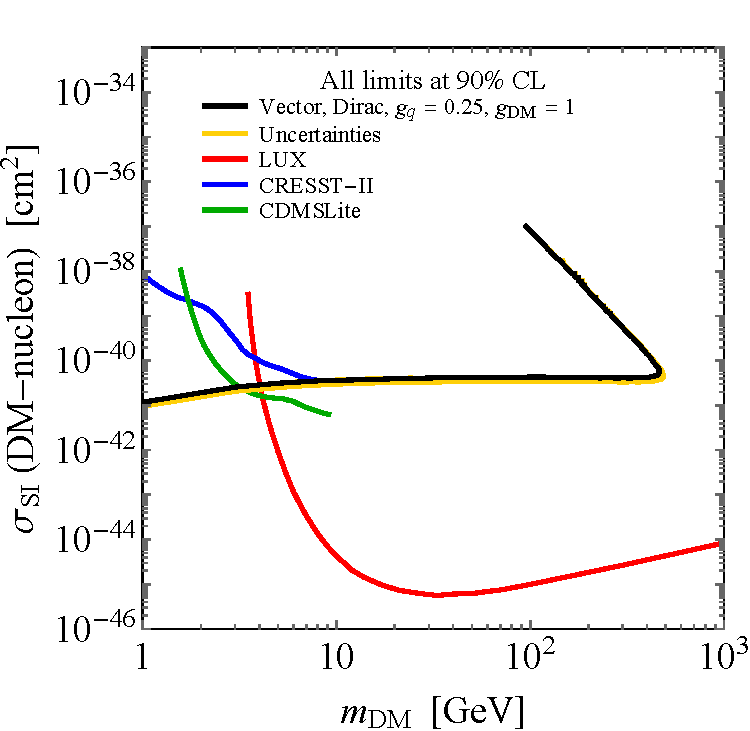
\includegraphics[width=1\textwidth]{figure2}
		\caption{~}
		\label{fig:SI}
	\end{subfigure}
	\qquad 
	\begin{subfigure}{0.45\textwidth}
		\centering
		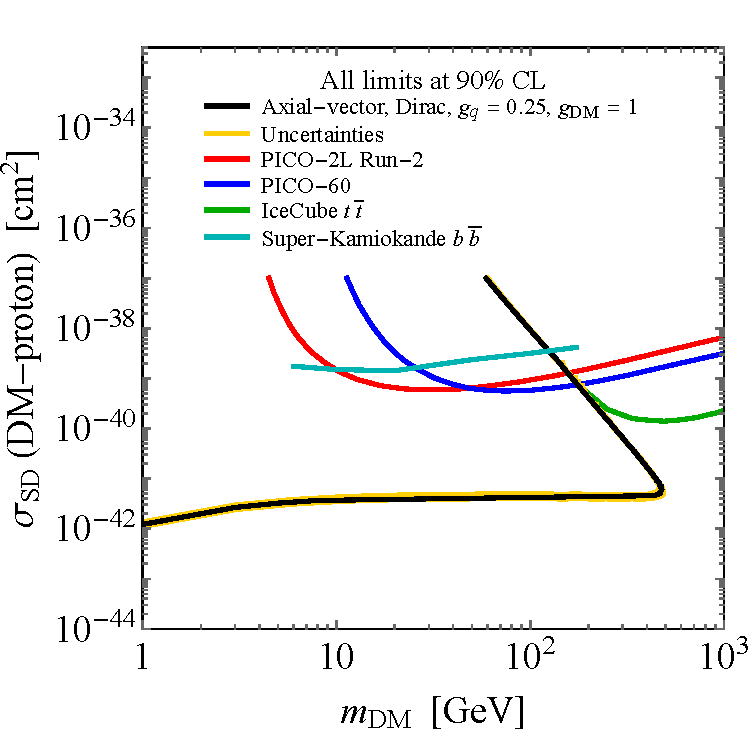
\includegraphics[width=1\textwidth]{figure3}
		\caption{~}
		\label{fig:SD}
	\end{subfigure}
	\caption{		
	A comparison of  LHC results to the  $\mDM$--$\hspace{0.25mm} \sigma_{\rm{SI}}$   (a) and  $\mDM$--$\hspace{0.25mm} \sigma_{\rm{SD}}$ (b) planes. Unlike in the mass-mass plane, the limits are shown at 90\%~CL. The LHC contour in the~SI~(SD) plane is for a vector (axial-vector) mediator, Dirac DM and couplings $\gq=0.25$ and $\gDM=1$. The LHC SI exclusion contour is compared with the LUX, CDMSLite and CRESST-II limits, which are the most constraining in the  shown mass range. The  SD exclusion contour constrains the DM-proton  cross section and is compared with limits from the PICO experiments, the IceCube limit for the $t\bar{t}$ annihilation channel and the Super-Kamiokande limit for the $b\bar{b}$ annihilation channel. The  depicted LHC results are intended for illustration only and are not based on real data.				 
	}   
	\label{fig:SISD}	
\end{figure}





\subsubsection{SI cases: Vector and scalar mediators}
\label{sub:spinindependent}

In general, the  SI DM-nucleon scattering  cross section takes the form
\begin{equation}
\sigma_{\rm{SI}}=\frac{f^2(\gq) \gDM^2 \mu^2_{n\chi}}{\pi \mmed^4}\,,
\end{equation}
where $\mu_{n\chi}= m_n \mDM/(m_n+\mDM)$ is the DM-nucleon reduced mass with $m_n \simeq 0.939 \, \mathrm{GeV}$ the nucleon mass. The mediator-nucleon coupling is $f(\gq)$ and depends on the mediator-quark couplings. For the interactions mediated by vector and scalar particles and for the recommended coupling choices, the difference between the proton and neutron  cross section is negligible. 
 
For the vector mediator, 
\begin{equation}
f(\gq) = 3 \hspace{0.25mm} \gq \,, 
\end{equation} 
and hence
\begin{align}
\label{eq:SI2MSDM}
 \sigma_{\rm{SI}} \simeq 6.9\times 10^{-41}~\mathrm{cm}^2\cdot\left(\frac{\gq \hspace{0.25mm} \gDM}{0.25}\right)^2\left( \frac{1 \, \mathrm{TeV}}{\mmed}\right)^4\left(\frac{\mu_{n\chi}}{1 \, \mathrm{GeV}} \right)^2\,.
\end{align}

For the simplified model with scalar mediator exchange we follow the recommendation of  ATLAS/CMS  DM Forum~\cite{Abercrombie:2015wmb} and assume that the scalar mediator couples to all quarks (like e.g.~the  SM Higgs). In general the formula for $f(\gq)$ is
\begin{equation}
\label{eq:fscalar}
f^{n,p}(\gq) = \frac{m_{n}}{v} \left[\sum_{q=u,d,s}f_q^{n,p} g_q + \frac{2}{27} \hspace{0.5mm} f^{n,p}_{\rm{TG}}\sum_{Q=c,b,t} g_Q \right]\,.
\end{equation}
Here $f^{n,p}_{\rm{TG}}=1-\sum_{q=u,d,s}f_q^{n,p}$. The state-of-the-art values for $f_q^{n,p}$ are from~\cite{Hoferichter:2015dsa} (for $f_u^{n,p}$ and $f_d^{n,p}$) and~\cite{Junnarkar:2013ac} (for $f_s^{n,p}$) and read  $f_u^{n}=0.019$, $f_d^{n}=0.045$ and $f_s^{n}=0.043$. The values for the proton are slightly different, but in practice the difference can be ignored. Substituting these values, we find that numerically
\begin{equation}
 f(\gq)  = 1.16 \cdot 10^{-3} \hspace{0.5mm} \gq \,,
\end{equation}
and therefore the size of a typical  cross section is
\begin{equation}
\sigma_{\rm{SI}} \simeq 6.9\times 10^{-43}~\mathrm{cm}^2\cdot\left(\frac{\gq \hspace{0.25mm} \gDM}{1}\right)^2\left( \frac{125 \, \mathrm{GeV}}{\mmed}\right)^4\left(\frac{\mu_{n\chi}}{1 \, \mathrm{GeV}} \right)^2\,.
\end{equation}


\subsubsection{SD case: Axial-vector mediator}
\label{sub:spindependent}

For the axial-vector mediator, the scattering is  SD and the corresponding  cross section can be written as
\begin{equation}
\sigma_{\rm{SD}}=\frac{3 \hspace{0.25mm} f^2(\gq) \gDM^2 \mu^2_{n\chi}}{\pi \mmed^4}\,.
\end{equation}
In general $f^{p,n}(\gq)$ differs for protons and neutrons and is given by
\begin{equation}
 f^{p,n}(\gq) = \Delta^{(p,n)}_u \, g_u + \Delta^{(p,n)}_d \, g_d + \Delta^{(p,n)}_s \, g_s \,,
\end{equation}
where $\Delta^{(p)}_u= \Delta^{(n)}_d = 0.84$, $\Delta^{(p)}_d = \Delta^{(n)}_u = -0.43$ and $\Delta_s=-0.09$ are the values recommended by  the Particle Data Group~\cite{Agashe:2014kda}. Other values are also used in the literature (see~e.g.~\cite{Ellis:2008hf}) and differ by up to~$\mathcal{O}(5\%)$.

Under the assumption that the coupling~$g_q$ is equal for all quarks, one finds 
\begin{equation}
f(\gq) = 0.32 \hspace{0.25mm} \gq \,,
\end{equation} 
and thus
\begin{align}
\label{eq:SD2MSDM}
 \sigma^{\rm{SD}} \simeq 2.4\times 10^{-42}~\mathrm{cm}^2\cdot\left(\frac{\gq \hspace{0.25mm} \gDM}{0.25}\right)^2\left( \frac{1 \, \mathrm{TeV}}{M_{\rm{med}}}\right)^4\left(\frac{\mu_{n\chi}}{1 \, \mathrm{GeV}} \right)^2\,.
\end{align}
We emphasise that the same result is obtained both for the  SD DM-proton scattering  cross section $\sigma^p_{\rm{SD}}$ and the  SD DM-neutron scattering  cross section $\sigma^n_{\rm{SD}}$. Using \eqref{eq:SD2MSDM} it is therefore possible to map collider results on both parameter planes conventionally shown by  DD  experiments. Should only one plot be required, we recommend comparing  the LHC results to  the DD  bounds on $\sigma^p_{\rm{SD}}$, which is typically more difficult to constrain.

In the future, it is desirable to consider not only the case $g_u = g_d = g_s$, but also the case $g_u = -g_d = -g_s$, which is well-motivated from embedding the simplified model in the SM gauge group and can be included without much additional effort. For $g_u = -g_d = -g_s$ one obtains approximately $f^p(\gq) = 1.36 \, g_u$ and $f^n(\gq) = - 1.18 \, g_u$, i.e.\ the DM-neutron  cross section is slightly smaller than the DM-proton  cross section.\footnote{LHC searches are only sensitive to the relative sign between $g_u$ and $g_d$ if both types of quarks are present in a single process (e.g.~$u \bar{d} \rightarrow u \bar{d} + \chi \bar{\chi}$ or $u \bar{u} \rightarrow d \bar{d} + \chi \bar{\chi}$). Such processes give a  subleading effect in mono-jet searches and are presently not included in the signal computation. As a result, the signal prediction for mono-jets turns out to be independent of the relative sign between the individual quark couplings~\cite{Haisch:2016usn}.}

\subsubsection{Neutrino observatories: IceCube and Super-Kamiokande}

The IceCube~\cite{Aartsen:2016exj} and Super-Kamiokande~\cite{Choi:2015ara} neutrino observatories are also able to constrain the~SI and SD cross sections. When DM particles elastically scatter with elements in the Sun, they can lose enough energy to become gravitationally bound. Self-annihilation of the DM particles produces neutrinos (either directly or in showering) that can be searched for in a neutrino observatory. When the DM capture and annihilation rates are in equilibrium, the neutrino flux depends only on the initial capture rate, which is determined by the SI or SD cross section~\cite{Silk:1985ax}.  

The IceCube and Super-Kamiokande limits on~$\sigma^p_{\rm{SD}}$ are of particular interest as they can be stronger than the corresponding bounds from DD experiments.  The former bounds are however more model dependent, since they depend on the particular DM annihilation channel.  For annihilation only into light quarks, the limits are weaker than DD experiments. For $m_b< m_\text{DM} < m_t$, on the other hand, the dominant annihilation channel of the axial-vector model is to $b \bar{b}$ and Super-Kamiokande sets more stringent constraints than DD experiments for $\mDM<10 \, \rm{GeV}$. For $m_\text{DM} > m_t$, the dominant annihilation channel is to~$t \bar{t}$ and the resulting constraints from IceCube are stronger than DD experiments. Both the Super-Kamiokande and IceCube limits can be shown together with other bounds on the SD DM-proton scattering cross section.  

While strong bounds are obtained for annihilation into bosons or leptons, these couplings are not present in the simplified models considered here. Therefore, we do not recommend showing the IceCube or Super-Kamiokande limits for annihilation into bosons or leptons. Note also that the IceCube bounds may be further modified if the DM particles can directly annihilate into the mediator (see the discussion in~\cite{Heisig:2015ira}). For $\mDM\lesssim4~\mathrm{GeV}$, the effects of DM evaporation from the Sun are important, so placing
limits on~$\sigma^p_{\rm{SD}}$ and~$\sigma_{\rm{SI}}$ from neutrinos coming from the Sun becomes very difficult in this low-mass regime 
(see~e.g.~\cite{Busoni:2013kaa}).


\subsection{ID experiments}
\label{sec:indirect}


For a  pseudo-scalar mediator, the rate at DD experiments is suppressed by additional velocity-dependent terms entering the  cross section. As a result,  DD experiments have very little sensitivity for this scenario and it is not worthwhile to compare  LHC results to the usual bounds on SI and SD  cross sections. Instead,  LHC bounds  can be compared against the limits from  ID experiments. 
For example, Fermi-LAT places 95\%~CL constraints on the self-annihilation  cross section from observations of dwarf spheroidal galaxies~\cite{Ackermann:2015zua}.\footnote{The galactic center is also potentially a promising DM target.  Current observations show an excess of gamma rays which are roughly consistent with a DM signal, but cannot be conclusively identified as such due to poorly understood astrophysical
backgrounds~\cite{TheFermi-LAT:2015kwa}.  The regions of simplified models capable of reproducing this excess are currently regions of particular interest
for collider and direct searches.} Limits are set on the  cross section $\sigv$ to annihilate to a single  particle-anti-particle final state. 

There are a number of subtleties when dealing with these limits. Firstly, all of the  bounds shown in~\cite{Ackermann:2015zua} are for a Majorana fermion. ID annihilation cross section limits for a Dirac fermion are larger by a factor of two and therefore need to be rescaled before they can be compared to the Dirac DM simplified model considered here. Secondly, the limits are for single  particle-anti-particle final states while models typically include more than one final state. For the  pseudo-scalar model, for example, DM annihilates to all quarks with branching ratios approximately proportional to $m_q^2$.
In practice, however, the gamma-ray flux that is observed from annihilating to different quarks (or gluons) is small~\cite{Cirelli:2010xx}. The~Fermi-LAT limits~\cite{Ackermann:2015zua} also demonstrate that there is a negligible difference between the limits on $\sigv$ in $u \bar{u}$ and $b \bar{b}$ final states. We therefore suggest to only show the bound on $u\bar{u}$ from Fermi-LAT in comparison with the calculated bound on the total annihilation cross section, as representative of the limits to final states involving linear combinations of different quarks or gluons. 

\begin{figure}[t!]
	\centering
	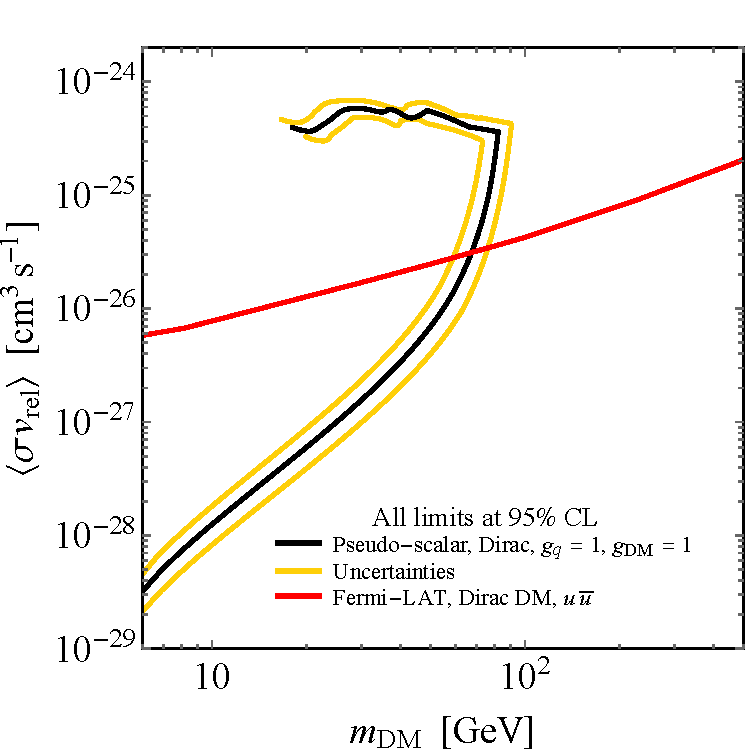
\includegraphics[width=0.6\textwidth]{figure4}
	\caption{A comparison of the  LHC result to the Fermi-LAT limit in the $\mDM$--$\sigv$  plane. Both limits are at 95\%~CL. The Fermi-LAT limit is for Dirac DM and assumes that the only annihilation channel is to $u \bar{u}$ quarks. The Fermi-LAT limits to other  quark-anti-quark annihilation channels will be similar. The LHC exclusion contour is for a  pseudo-scalar mediator, Dirac DM and couplings $\gq=1$ and $\gDM=1$.  The shown  LHC results are intended for illustration only and are not based on real data.}
	\label{fig:ID}
\end{figure}


The annihilation  cross section into a $q \bar{q}$ final state is (see~e.g.~\cite{Buchmueller:2015eea} for a recent example)  
\begin{equation} \label{eq:qqann}
 \langle \sigma v_{\rm{rel}}\rangle_q =\frac{3 \hspace{0.25mm} m_q^2}{2 \pi v^2} \hspace{0.25mm} \frac{\gq^2  \hspace{0.25mm}  \gDM^2  \hspace{0.25mm}  \mDM^2}{(\mmed^2-4 \mDM^2)^2+\mmed^2 \Gamma_{\rm med}^2} \, \sqrt{1-\frac{m_q^2}{\mDM^2}}\,,
\end{equation}
where  $\Gamma_{\rm med}$ is the total width of the mediator (see  Section~\ref{sub:smodels}). Similarly, the annihilation  cross section into a pair of gluons is given by
\begin{equation} \label{eq:ggann}
\langle \sigma v_{\rm{rel}}\rangle_g =\frac{\alpha_s^2}{2 \hspace{0.25mm}  \pi^3 v^2}\hspace{0.25mm} \frac{\gq^2 \hspace{0.25mm} \gDM^2}{(\mmed^2-4 \mDM^2)^2+\mmed^2 \Gamma_{\rm med}^2} \, \left|\sum_q m_q^2 \hspace{0.5mm} f_\text{pseudo-scalar}\left(\frac{m_q^2}{m_\chi^2}\right)\right|^2\,,
\end{equation}
where $f_\text{pseudo-scalar} (\tau)$ 
has been defined in 
(\ref{eq:fPS}) and $\alpha_s$ is the strong coupling constant, which we recommend to evaluate at the scale $\mu = 2 \mDM$. The  total cross section is then given by  the sum of the quark and gluon channels (\ref{eq:qqann}) and (\ref{eq:ggann}) as well as any annihilation channels into on-shell
mediators which are kinematically allowed and are not suppressed by the small relative velocities of DM in the galactic halo.

Figure~\ref{fig:ID} depicts the translation of  LHC bounds   for a pseudo-scalar mediator to the  $\mDM$--$\sigv$ plane. As with the other plots, we recommend to specify explicitly details including the mediator and DM type, the choices of couplings and the CL of the exclusion limits. It is also important to emphasise that the  ID limit is for Dirac DM instead of Majorana DM as assumed in the Fermi-LAT publication.  Since the  LHC exclusion contour in the mass-mass plane passes through two values of $\mmed$,  the LHC limit shows a similar turnover behaviour in the  $\mDM$--$\sigv$ plane.  In Figure~\ref{fig:ID} we have depicted both branches of the exclusion contour that are obtained for fixed DM mass $\mDM$. 
It may also be desirable to show the values of~$\sigv$ in Figure~\ref{fig:ID} that produce the observed relic density.  A standard reference providing the values of~$\sigv$ as a function of~$\mDM$ is~\cite{Steigman:2012nb}. We reemphasise the point made in~\cite{Steigman:2012nb} that their displayed values of~$\sigv$ should be multiplied by a factor of two for Dirac DM.

To conclude this section, we emphasise that 
translating DD or ID searches into bounds on the DM-nucleon scattering  cross section  or the DM self-annihilation cross section plane always require an assumption on the density of DM particles. In particular, it is always assumed that the particle under consideration constitutes all of the DM in the Universe. If $\chi$ is only one out of several DM sub-components, bounds from  DD and ID experiments would become weaker, while  the LHC bounds  remain unchanged.

